\documentclass[multi,crop,tikz,border=0pt,12pt]{standalone}

\usepackage{latexsym,mathtools}
\def\lineThickness{.7}
\usetikzlibrary{decorations.pathmorphing,shapes}

\definecolor{lightblue}{rgb}{0.8,0.8,1.0}

\newcommand{\dn}{\downarrow}
\newcommand{\dns}{\downarrow}	%Strict down-arrow for colorings
\newcommand{\dnw}{\Downarrow}	%Weak downarrow for colorings

\newcommand{\estep}{\texttt{e}}
\newcommand{\dstep}{\texttt{d}}
\newcommand{\nstep}{\texttt{n}}
\newcommand{\bs}{{\kern-.08em\texttt{.}\kern-.13em}} %bounce separator


%%%%%%%%%%%%%%%%%%%%%%%%%%%%%%%%%%%%%%%%%%%%%%%%%%%%%%%%%%%%%%%%%%%%%%%%%%
%% TIKZ CODE
%%%%%%%%%%%%%%%%%%%%%%%%%%%%%%%%%%%%%%%%%%%%%%%%%%%%%%%%%%%%%%%%%%%%%%%%%%

\tikzset{every picture/.append style={
	scale=1,
	baseline=(current bounding box.center),
	x=1em,
	y=1em,
	thinLine/.style={line width=\lineThickness pt},
	snaking/.style={decorate,decoration={zigzag,segment length=1.0mm,amplitude=0.15mm}},
	thickLine/.style={line width=2*\lineThickness pt,line join=round},
	fillGrey/.style={fill=black!10},
	entries/.style={xshift=-0.5em,yshift=-0.5em,font=\small},
	circled/.style={circle,draw,inner sep=0pt,minimum size=1em},
	mydot/.style={circle,fill=black,inner sep=0pt,minimum size=1mm}
  }
}

\tikzset{relationDiagram/.append style={
	x=0.8em,
	y=0.8em,
	entries/.style={xshift=-0.4em,yshift=-0.4em,font=\small},
}}

\tikzset{
	redBounceSS/.pic = {
		code {
			\draw[red,thickLine,->] (6,9)--(6,6)--(3,6);
		}
	},
	redBounceLS/.pic = {
		code {
			\draw[red,thickLine,->] (6,10)--(6,6)--(3,6);
		}
	},
	redBounceSL/.pic = {
		code {
			\draw[red,thickLine,->] (6,9)--(6,6)--(2,6);
		}
	},
	redBounceLL/.pic = {
		code {
			\draw[red,thickLine,->] (6,10)--(6,6)--(2,6);
		}
	},
	redBounceBigStart/.pic = {
		code {
			\draw[red,thickLine,->] (6,10)--(6,6)--(2,6);
		}
	},
	redBounceBigRest/.pic = {
		code {
			\draw[red,thickLine,->] (2,6)--(2,2)--(0.2,2);
		}
	},
	xyEdge/.pic = {
		code {
			\draw[entries] (6,7) node {#1};
		}
	},
	xzEdge/.pic = {
		code {
			\draw[entries] (6,10) node {#1};
		}
	},
	yzEdge/.pic = {
		code {
			\draw[entries] (7,10) node {#1};
		}
	},
	vxEdge/.pic = {
		code {
			\draw[entries] (2,6) node {#1};
		}
	},
	vyEdge/.pic = {
		code {
			\draw[entries] (2,7) node {#1};
		}
	},
	wxEdge/.pic = {
		code {
			\draw[entries] (3,6) node {#1};
		}
	},
	wyEdge/.pic = {
		code {
			\draw[entries] (3,7) node {#1};
		}
	},
	wyGray/.pic = {
		code {
			\fill[fillGrey] (1.9,6)--(3,6)--(3,7.1)--(1.9,7.1)--cycle;
			\draw (2,6)--(3,6)--(3,7);
		}
	},
	vxGray/.pic = {
		code {
			\fill[fillGrey] (0.9,5)--(2,5)--(2,6.1)--(0.9,6.1)--cycle;
			\draw (1,5)--(2,5)--(2,6);
		}
	},
	wxyGray/.pic = {
		code {
			\fill[fillGrey] (1.9,5)--(3,5)--(3,7.1)--(1.9,7.1)--cycle;
			\draw (2,5)--(3,5)--(3,7);
		}
	},
	xzGray/.pic = {
		code {
			\fill[fillGrey] (4.9,9)--(6,9)--(6,10)--(4.9,10)--cycle;
			\draw (5,9)--(6,9)--(6,10);
		}
	},
	xyzGray/.pic = {
		code {
			\fill[fillGrey] (4.9,9)--(7,9)--(7,10)--(4.9,10)--cycle;
			\draw (5,9)--(7,9)--(7,10);
		}
	}
}

\tikzset{
	basicPathBig/.pic = {
	code {
	\fill[fillGrey] (0,1)--(0,10)--(9,10);
	\fill[fill=white] 
	(0,0)--(0,4)--(1,5)--(1,6)--(2,6)--(2,7)--(3,7)
	--(5,9)--(5,10)--(9,10)--(9,9)--(7,7)--(6,7)
	--(6,6)--(5,6)--(5,5)--(3,3)--(2,3)--(2,2)--(1,1)--(0,0);
	
	%Default edge
	\draw (1,5)--(1,6)--(2,6)--(2,7)--(3,7);
	\draw (6,9.98)--(7,9.98);
	
	\draw[snaking]
	(9,9)--(7,7)--(6,7)--(6,6) 
	(5,5)--(3,3)
	(1,1)--(0,0)
	(0,4)--(1,5)
	(3,7)--(5,9);
	
	%Diag-thick
	\draw[thickLine] 
	(7,7)--(6,7)--(6,6)--(5,6)--(5,5)
	(3,3)--(2,3)--(2,2)--(1,2)--(1,1)
	(9,9)--(9,10)--(10,10);
	
	\draw[entries]
	(2, 2)node{$v$}
	(3, 3)node{$w$}
	(6, 6)node{$x$}
	(7, 7)node{$y$}
	(10, 10)node{$z$};
}}}

\tikzset{
	basicPath/.pic = {
	code {
	
	\fill[fillGrey] (1,2)--(1,10)--(9,10);
	\fill[fill=white] 
	(1,1)--(1,5)--(2,5)--(2,6)--(2,6)--(2,7)--(3,7)
	--(5,9)--(5,10)--(9,10)--(9,9)--(7,7)--(6,7)
	--(6,6)--(5,6)--(5,5)--(3,3)--(2,3)--(2,2)--(1,1);

	\draw[snaking]
 	(9,9)--(7,7) 
	(5,5)--(3,3)
	(2,2)--(1,1)
	(3,7)--(5,9);
	
	\draw (2,5)--(2,7)--(3,7);
	\draw (6,9.98)--(7,9.98);
	
	%Diag-thick
	\draw[black,thickLine] 
	(7,7)--(6,7)--(6,6)--(5,6)--(5,5)
	(3,3)--(2,3)--(2,2)
	(9,9)--(9,10)--(10,10);

	\draw[entries]
	(3, 3)node{$w$}
	(6, 6)node{$x$}
	(7, 7)node{$y$}
	(10, 10)node{$z$};
}}}

%%%%%%%%%%%%%%%%%%%%%%%%%%%%%%%%%%%%%%%%%%%%%%%%%%%%%%%%%%%%%%%%%%%%%%%%%%
%% END TIKZ CODE
%%%%%%%%%%%%%%%%%%%%%%%%%%%%%%%%%%%%%%%%%%%%%%%%%%%%%%%%%%%%%%%%%%%%%%%%%%

\begin{document}

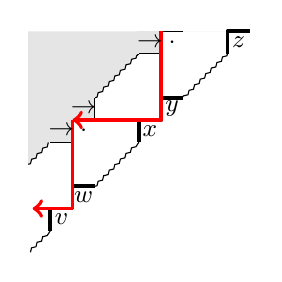
\begin{tikzpicture}[relationDiagram]
\draw pic {basicPathBig};
\draw pic {xzGray};
\draw pic {wyGray};
\draw pic {vxGray};
\draw pic {redBounceBigStart};
\draw pic {redBounceBigRest};
\draw pic {wxEdge=$\cdot$};
\draw pic {yzEdge=$\cdot$};
\draw pic {xzEdge=$\to$};
\draw pic {vxEdge=$\to$};
\draw pic {wyEdge=$\to$};
\end{tikzpicture}

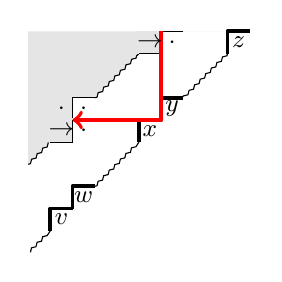
\begin{tikzpicture}[relationDiagram]
\draw pic {basicPathBig};
\draw pic {xzGray};
\draw pic {vxGray};
\draw pic {redBounceBigStart};
\draw pic {wxEdge=$\cdot$};
\draw pic {yzEdge=$\cdot$};
\draw pic {vyEdge=$\cdot$};
\draw pic {vxEdge=$\to$};
\draw pic {xzEdge=$\to$};
\draw pic {wyEdge=$\cdot$};
\end{tikzpicture}

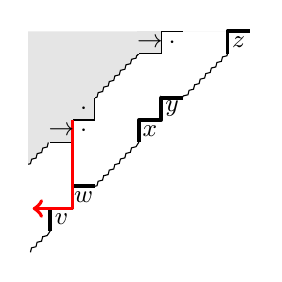
\begin{tikzpicture}[relationDiagram]
\draw pic {basicPathBig};
\draw pic {xzGray};
\draw pic {wyGray};
\draw pic {vxGray};
\draw pic {redBounceBigRest};
\draw pic {wxEdge=$\cdot$};
\draw pic {yzEdge=$\cdot$};
\draw pic {xzEdge=$\to$};
\draw pic {vxEdge=$\to$};
\draw pic {wyEdge=$\cdot$};
\end{tikzpicture}







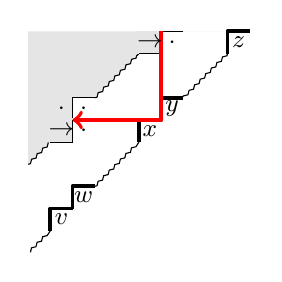
\begin{tikzpicture}[relationDiagram]
\draw pic {basicPathBig};
\draw pic {xzGray};
\draw pic {vxGray};
\draw pic {redBounceBigStart};
\draw pic {wxEdge=$\cdot$};
\draw pic {yzEdge=$\cdot$};
\draw pic {vyEdge=$\cdot$};
\draw pic {vxEdge=$\to$};
\draw pic {xzEdge=$\to$};
\draw pic {wyEdge=$\cdot$};
\end{tikzpicture}

 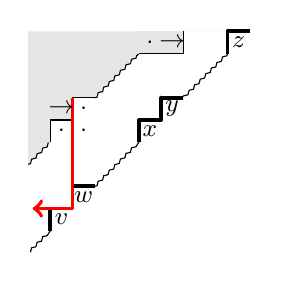
\begin{tikzpicture}[relationDiagram]
\draw pic {basicPathBig};
\draw pic {xyzGray};
\draw[red,thickLine] (2,7)--(2,6);
\draw pic {redBounceBigRest};
\draw pic {wxEdge=$\cdot$};
\draw pic {yzEdge=$\to$};
\draw pic {vyEdge=$\to$};
\draw pic {vxEdge=$\cdot$};
\draw pic {xzEdge=$\cdot$};
\draw pic {wyEdge=$\cdot$};
\end{tikzpicture}

 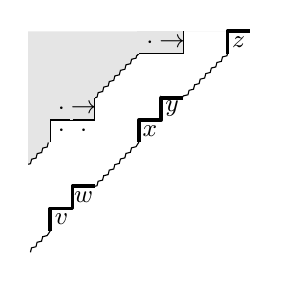
\begin{tikzpicture}[relationDiagram]
\draw pic {basicPathBig};
\draw pic {xyzGray};
\draw pic {wyGray};
\draw pic {wxEdge=$\cdot$};
\draw pic {yzEdge=$\to$};
\draw pic {vyEdge=$\cdot$};
\draw pic {vxEdge=$\cdot$};
\draw pic {xzEdge=$\cdot$};
\draw pic {wyEdge=$\to$};
\end{tikzpicture}







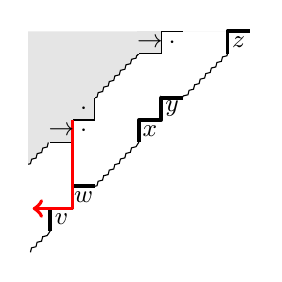
\begin{tikzpicture}[relationDiagram]
\draw pic {basicPathBig};
\draw pic {xzGray};
\draw pic {wyGray};
\draw pic {vxGray};
\draw pic {redBounceBigRest};
\draw pic {wxEdge=$\cdot$};
\draw pic {yzEdge=$\cdot$};
\draw pic {xzEdge=$\to$};
\draw pic {vxEdge=$\to$};
\draw pic {wyEdge=$\cdot$};
\end{tikzpicture}

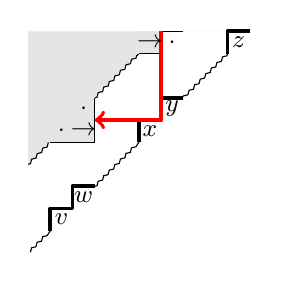
\begin{tikzpicture}[relationDiagram]
\draw pic {basicPathBig};
\draw pic {xzGray};
\draw pic {vxGray};
\draw pic {wxyGray};
\draw pic {redBounceLS};
\draw pic {vxEdge=$\cdot$};
\draw pic {wxEdge=$\to$};
\draw pic {yzEdge=$\cdot$};
\draw pic {xzEdge=$\to$};
\draw pic {wyEdge=$\cdot$};
\end{tikzpicture}

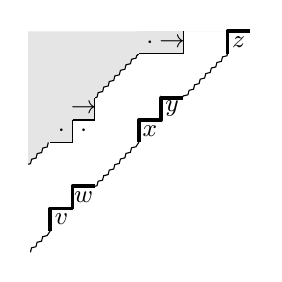
\begin{tikzpicture}[relationDiagram]
\draw pic {basicPathBig};
\draw pic {xyzGray};
\draw pic {vxGray};
\draw pic {wyGray};
\draw pic {vxEdge=$\cdot$};
\draw pic {wxEdge=$\cdot$};
\draw pic {xzEdge=$\cdot$};
\draw pic {yzEdge=$\to$};
\draw pic {wyEdge=$\to$};
\end{tikzpicture}


%%%%%%%%%%%%%%%%%%%%%%%%%%%%%%%%%%%%%%%%%%%%%%%%%%%%%%%%
% COLORING FIGS: Swap map and bounceI
%%%%%%%%%%%%%%%%%%%%%%%%%%%%%%%%%%%%%%%%%%%%%%%%%%%%%%%%

% Pic # 11
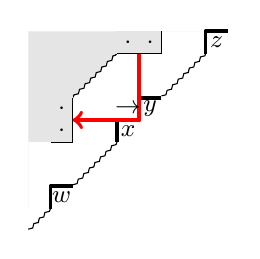
\begin{tikzpicture}[relationDiagram]
\draw pic {basicPath};
\draw pic {xyzGray};
\draw pic {wxyGray};
\draw pic {redBounceSS};
\draw pic {wxEdge=$\cdot$};
\draw pic {wyEdge=$\cdot$};
\draw pic {xzEdge=$\cdot$};
\draw pic {yzEdge=$\cdot$};
\draw pic {xyEdge=$\to$};
\end{tikzpicture}

% Pic # 12
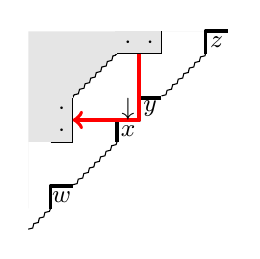
\begin{tikzpicture}[relationDiagram]
\draw pic {basicPath};
\draw pic {xyzGray};
\draw pic {wxyGray};
\draw pic {redBounceSS};
\draw pic {wxEdge=$\cdot$};
\draw pic {wyEdge=$\cdot$};
\draw pic {xzEdge=$\cdot$};
\draw pic {yzEdge=$\cdot$};
\draw pic {xyEdge=$\dn$};
\end{tikzpicture}


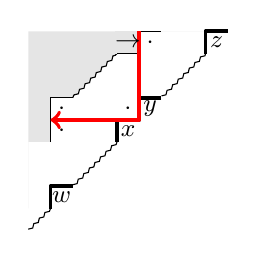
\begin{tikzpicture}[relationDiagram]
\draw pic {basicPath};
\draw pic {xzGray};
\draw pic {redBounceLL};
\draw pic {wxEdge=$\cdot$};
\draw pic {wyEdge=$\cdot$};
\draw pic {xzEdge=$\to$};
\draw pic {yzEdge=$\cdot$};
\draw pic {xyEdge=$\cdot$};
\end{tikzpicture}

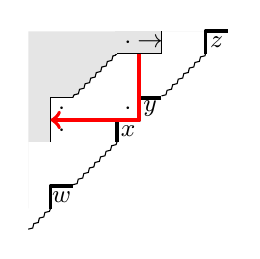
\begin{tikzpicture}[relationDiagram]
\draw pic {basicPath};
\draw pic {xyzGray};
\draw pic {redBounceSL};
\draw pic {wxEdge=$\cdot$};
\draw pic {wyEdge=$\cdot$};
\draw pic {xzEdge=$\cdot$};
\draw pic {yzEdge=$\to$};
\draw pic {xyEdge=$\cdot$};
\end{tikzpicture}

\end{document}
